% -----------------------------------------------
% Template for ISMIR 2013
% (based on earlier ISMIR templates)
% -----------------------------------------------

\documentclass{article}
\usepackage[utf8]{inputenc}
\usepackage{ismir2013,amsmath,cite}
\usepackage{graphicx}

% For Graphs
\usepackage{tikz}
\usetikzlibrary{shapes,arrows}
\usetikzlibrary{calc}
\usepackage{caption}
\usepackage{subcaption}

%For Tables
\usepackage{booktabs}
\usepackage{graphicx}
%\usepackage[showframe]{geometry}

% Title.
% ------
\title{CSC 475 Final Project: Automatic Chord Estimation Using SciKit Learn}

% Three addresses
% --------------
\threeauthors{Lee Gauthier} {\tt lgauthie@uvic.ca}
             {Robert Janzen} {\tt rjanzen@uvic.ca}
             {Sondra Moyls} {\tt smoyls@uvic.ca}

\begin{document}
%
\maketitle
%


\section{Abstract}\label{sec:desoutline}
This project aims to investigate and evaluate some of the current strategies
for automatic chord estimation. We present a simple HMM-based mode that uses
the SciKit Learn framework for detecting chords from audio signals using beat
synchronous chroma vectors.  SciKit learn is an open source toolkit in Python 
for machine learning. We evaluate the effectiveness of Harmonic/Percussive 
Sound Separation (HPSS) as a preprocessing step by
comparing the results of an unaltered data set to the results of a dataset that
has undergone HPSS preprocessing, and find that HPSS is a valuable
preprocessing step prior to extracting chroma vectors.

\section{Introduction}\label{sec:intro}

Chords describe the harmonic content of a piece of music. Automatic estimation
of chords has many applications in music information retrieval and music
annotation. For example, automatic chord estimation may be used to infer
genre and emotional content (minor, sad; major, happy) of a piece, or to
identify songs of similar compositional form.  It has also been used successfully in
detecting cover-songs~\cite{Papadopoulos:18}.

Automatic chord detection has been a MIREX task since 2008, and has since seen
increased improvement, with submissions in 2012 surpassing 72 percent accuracy
on unseen data~\cite{McVicar:00}. Hidden Markov Models have been used as a
successful modeling strategy in a number of automatic chord estimation models,
including~\cite{Ueda:01}~\cite{Lee:15}~\cite{Ueda:19} and
\cite{Papadopoulos:18}. All of these models use chroma vectors (Pitch Class
Profiles) at the feature extraction phase, which represent the pitch content
of a song for each sampled window. Each chroma vector is a real valued vector
which contains the salience of each of the pitch classes (A, A\# \dots G, G\#) for a
given time window.~\cite{McVicar:00},~\cite{Lee:15},~\cite{Papadopoulos:18},
and\cite{Zenz:20} have all found that chroma extraction on beats improves
results, as chords are most stable between beats.

Another method to improve the resolution of chromagrams is filtering out
transient and percussive information that does not contribute to the harmonic
content, but may add noise to the extracted chromagram. A simple technique for
this is to filter the frequencies where chromas are extracted so that they are
restricted to the range with the most pitch content. Another is to suppress
harmonic and percussive sounds using harmonic/percussive sound separation
(HPSS).  It has been noted that applying this preprocessing step can greatly
improve chord estimation accuracy ~\cite{Reed:09}.

\section{Overview}\label{sec:approch}

For this project we used part of the annotated Billboard 100 data set. Our data
set included audio files for approximately 650 audio files from the Billboard
top 100 chart between the years 1958 and 1991. Each song in the data set includes beat by
beat chord annotation~\cite{Burgoyne:07}. The chords are labeled as either maj,
min, aug, dim, sus2, sus4, or N, where N imply no chord is present. A
distinction is made between enharmonic labels (for example both G\# and Ab
occur in the annotations), for a total of 128 chord labels.

For our the scope of our project we reduced this number by combining enharmonic 
labels and reassigning the chord labels into two classes, major and
minor, as seen in Figure~\ref{fig:chordlabs}. Combined with the no chord label,
we considered 25 distinct chord labels to train and test our model.

\begin{figure}
\begin{center}
	\resizebox{0.4\textwidth}{!}{%
	\begin{tabular}{l c}
	\toprule
	 Original Chord Labels        & Treated As   \\ \midrule
	 Maj, Aug, sus4, sus2         & Maj           \\ \midrule
	 min, dim                     & min           \\
	\bottomrule
	\end{tabular}
	}
\caption{Chord Labels}
\label{fig:chordlabs}
\end{center}
\end{figure}

We used two sets of audio data: one unprocessed, and one preprocessed by
performing harmonic percussive source separation (HPSS). Each audio file was
mixed to mono to reduce processing time. Then, chormagram extraction was
performed on the two audio datasets at intervals corresponding to the beat
information in the annotated data, and only considered information from octaves
1 through 5 (approximately 60--1000Hz).

After extracting the chromagram for each song in the data set, 63 of the tracks
were randomly chosen using the random function in Python and kept as testing
data. The rest of the data was used to train our HMM model.

A full overview of our proposed model can be seen in Figure~\ref{fig:overview}.

% Define block style
\tikzstyle{block} = [rectangle, draw, fill=blue!20,
    text width=7em, text centered, rounded corners, minimum height=4em]
\tikzstyle{line} = [draw, -latex']

\begin{figure}
\begin{tikzpicture}[node distance=3cm]
    % Place nodes
    \node [block] (init) {Billboard Data Set};
    \node [block, below left of= init] (chordlabel) {Labeled Chords By Beat (.txt)};
    \node [block, below right of= init] (audio) {Audio (.wav)};
    \node [block, below of= chordlabel] (chordname) {Chord Names at Beat Times};
    \node [block, below of= audio] (chroma) {12-bin chroma features};
    \coordinate (Middle) at ($(chordlabel)!0.5!(chroma)$);
    \node [block, below of  =Middle, yshift=-1cm] (hmm) {HMM};
    \node [below of  =Middle] (train) {Training};
    % Draw edges
    \path [line] (init) -- (audio);
    \path [line] (init) -- (chordlabel);
    \path [line] (chordlabel) -- node {Analyze Groud Truth} (chordname);
    \path [line] (audio) -- node {Analyze Chroma} (chroma);
    \path [line] (chroma) -- (hmm);
    \path [line] (chordname) -- (hmm);

\end{tikzpicture}
\caption{System Overview}
\label{fig:overview}
\end{figure}

\section{Model}

\subsection{PreProcessing}

In a spectrogram, the harmonic components of a musical signal have a stable
pitch and form parallel ridges along the time axis. Transient sounds distribute
their frequency content across the entire spectrum and occur during short time
frames, which can be seen as spikes in the frequency axis. The end product of
HPSS is two signals, one with mostly harmonic content, the other with
percussive sounds which is obtained by complementary diffusion on the
spectrogram.

HPSS was completed using Python code provided by~\cite{librosa:24}. To separate
the frequency content produced by percussive elements from the harmonic
elements, median filtering is applied.  It works by replacing each frequency
bin with the median of the values in the surrounding bins~\cite{FitzGerald:11}.
In our implementation an $l$ size of 23 provided the best result given the
broad range of audio styles in the Billboard dataset. When $l$ was larger than
40, the attack of harmonic components became too slow, which is valuable
information during chroma extraction.

$$ y(n) = median \left \{x(n-k:n+k),l = (l-2)/2  \right \} $$

The percussive suppressed spectrogram (the harmonic information) is then used
to create a mask which is applied to the original spectrogram. A soft mask
based on Wiener Filtering is used with a p-value of 2. From here the inverse
short time fourier transform is used to obtain the harmonic audio. Our system
only makes use of the harmonics, however, the  separated percussive audio could
be a useful pre-processing step for beat extraction in future work.

\begin{figure}
   \centering
    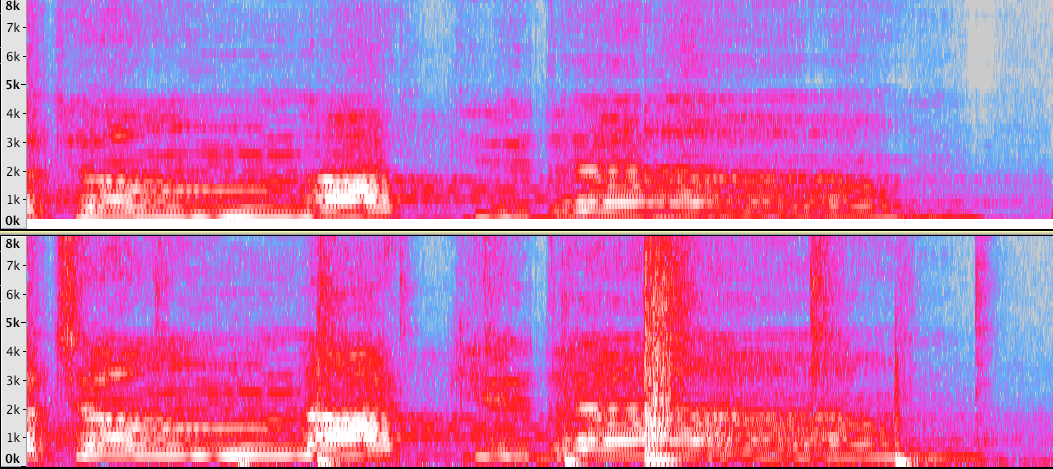
\includegraphics[width=0.5\textwidth]{hpssspec.png}
   \caption{Top: Harmonic result of HPSS, Bottom: Original Signal}\label{fig:HPSS}
\end{figure}


\begin{figure*}
	\resizebox{\textwidth}{!}{%
	\begin{tabular}{l c c c}
	\toprule
                               & 64 Test Set Avg & All Songs Test Set Avg & All Songs Test Set Max  \\ \midrule
	Non-Processed              & 1.0\%           & 1.0\%                  & 20.7\%   \\
	HPSS                       & 1.5\%           & 1.0\%                  & 19.9\%   \\
	Non-Processed --- 2 Iter    & 3.2\%           & 2.9\%                  & 44.7\%   \\
	HPSS --- 2 Iter             & 3.7\%           & 3.4\%                  & 60.5\%   \\
	Non-Processed --- 10 Iter   & 3.5\%           & 3.2\%                  & 38.9\%   \\
	HPSS --- 10 Iter            & 4.1\%           & 4.1\%                  & 36.5\%   \\
	Non-Processed --- 100 Iter  & 4.2\%           & 3.9\%                  & 17.1\%   \\
	HPSS --- 100 Iter           & 5.1\%           & 4.6\%                  & 18.0\%   \\
	100 Songs --- 500 Iter      & 5.5\%           & 5.3\%                  & 20.1\%   \\
	HPSS 100 Songs --- 500 Iter & 6.2\%           & 6.4\%                  & 25.8\%   \\
	\bottomrule
	\end{tabular}
	}
\caption{Results Table}
\label{fig:resulttable}
\end{figure*}

\cite{Ueda:19} discusses a model very similar to our goals. Using the
Beatles annotated data set, a 74.24 percent chord recognition rate was achieved
without HPSS, and a 78.48 percent chord recognition rate was achieved with it.
Our results also show similar gains after using the preprocessed audio.

\subsection{Chromogram Computation}

\begin{figure*}
	\centering
    \begin{subfigure}[b]{0.47\textwidth}
        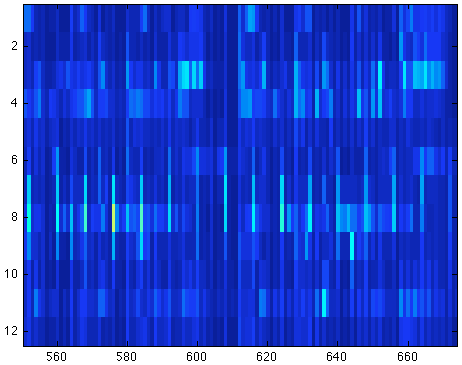
\includegraphics[width=\textwidth]{187.png}
        \caption{Extracted Chroma Vector}\label{fig:ChromaNorm}
    \end{subfigure}
    \begin{subfigure}[b]{0.47\textwidth}
        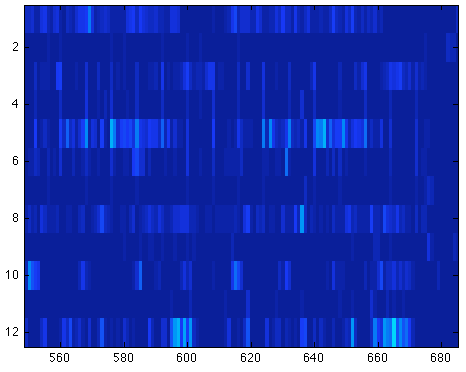
\includegraphics[width=\textwidth]{187h.png}
        \caption{Extracted Chroma Vector after HPSS}\label{fig:ChromaHPSS}
    \end{subfigure}
\end{figure*}

To compute the 12-dimensional chroma vectors (or Pitch Class Profiles), we used
the Chroma method available in Marsyas, and restricted the frequencies between
Octave 1 and 5 (\~60--1000Hz).

Because most chord transitions occur on beats, extracting chorma information for
windows corresponding to each beat has shown to be beneficial to creating an
more accurate automatic chord estimation model. For example, in~\cite{Zenz:20},
extracting chroma vectors on beats improved the results by 6 percent. This method 
exploits the stability of chords between beats, and reduces the overall computational 
cost by reducing the total number of windows \cite{McVicor:00}. Because the Billboard 
data is annotation at beat times, this approach naturally lines up with our ground truth data.

Two sets of chromagrams were calculated for our dataset, one set with HPSS
applied to the audio, and one set without. A comparison of the resulting
chromagrams for part of the song `Help Is On The Way' by the Little River Band
can be seen in figures~\ref{fig:ChromaNorm} and~\ref{fig:ChromaHPSS}
respectively. In these figures, the y-axis corresponds to the chord labels
$ C(1), C\#(2), D(3), $ etc. It's clear to see that after the HPSS processing, the
chromas become much cleaner.

\subsection{Hidden Markov Models}

Hidden Markov Models (HMMs) are a probabalistic model for time-series data. Because chord
sequences are continuous,  Hidden Markov Models have become a common method for
for automatic chord estimation and adapts well to the continuous nature of chord sequences. 
In this model, a given chord depends only on the previous chord predicted while all the other chords 
are hidden. For each song in our data set, the set of chorma vectors are the observations,
while the chord labels are our states.

To create our model, we used the SciKit Learn framework; however, because the
framework is designed for unsupervised learning, we needed to calculate the
prior probability, covariance and mean of the chromas  (which are represented as
a 12-dimensional Gaussian distribution) to construct our initial transition
matrix.  This transition matrix represents the probability of one chord
transitioning to another, independent of the previous chords.  This was based
off of Dan Ellis' Matlab code available through LabROSA\@. Due to the large size
of our dataset, using Matlab was infeasible for processing time, so this was
rewritten into Python to be fed into SciKit's GaussianHMM model.

SciKit uses the Expectation Maximization (EM) algorithm to train the model and the 
Viterbi algorithm to predict the most likely chord progression given a sequence
of chroma vectors. The number of iterations for the EM algorithm is specified by the user. For
comparison, we also trained our unprocessed and our processed data using 2,
10, and 100 iterations of the unsupervised EM algorithm. We also ran a random 
subset of 100 songs from each data set though 500 iterations.

To test our model, we used two training and testing sets. First, the model was trained
and tested with all of the data. Secondly, 63 random songs were removed from the data
set and reserved for testing while the rest were used to training. 

\begin{figure}
   \centering
   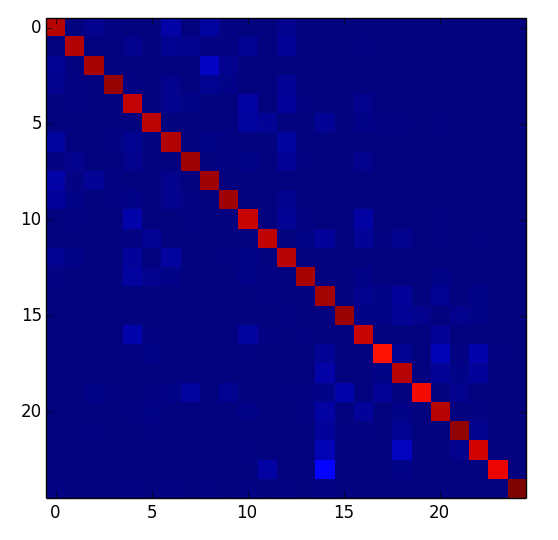
\includegraphics[width=0.4\textwidth]{trans-h.png}
   \caption{Initial Transition Matrix}\label{fig:transmath}
\end{figure}

\subsection{Evaluation}

Despite creating the initial values to train the data with supervised learning,
we were unable to optimize the Viterbi algorithm to find the optimal path
through the states. Because it uses recognition, and not a forced alignment
technique, the algorithm assumes any chord may follow another, even if those
state transitions never appeared in the training data.~\cite{Danellis:23}
discusses the impact of this optimization on an EM-Trained HMM chord model.
Without the forced alignment, results using chromagrams were as low as 10
percent on a small set of Beatles song data. When forced alignment was used,
and the algorithm only assumed progressions in the test data were valid,
results on the same test set increased by over 16 percent.

% TODO: EDIT ME

\section{Conclusion and Future Work}

We have introduced a simple beat-synchronous automatic chord estimation model
and evaluated the effectiveness of HPSS as a preprocessing step.

One preprocessing step that we have not considered in this paper is tuning.
Because tuning pitch may differ between recordings, it may be necessary to
consider different candidate chroma vectors. McVicar\cite{McVicar:00} suggests that
tuning using Harte's tuning algorithm is a staple of most modern algorithms.
Some older papers such as~\cite{Zenz:20} mention micro-tuning of the human
voice as well as percussive sounds as sources of classification error, so
tuning algorithms may be worth investigating as a future preprocessing step in
addition to HPSS\@.

The estimation model could also be improved by taking into account more
information about the music context. For example, information about key could
be used to choose a reasonable starting chord, or limit the choices of chords
for the current song. Limiting the chord choices will run into problems if the
song relies on out of key chords, or has a key change at any point. Information
about the time signature of a song could be used to decide when chord changes
occur. A simple way to add this in would be to penalize chords from changing on
weak beats. In both cases this extra information could be encoded in a Markov
Logic Network as suggested in~\cite{Papadopoulus:04}.

Each song in the Billboard dataset also includes key information. It is
possible to use the HMM model to simultaneously estimate the chords and the key
of an input audio file~\cite{McVicar:00}, so a future implementation may use
this data to predict key information as well as chords.

\begin{thebibliography}{citations}

\bibitem{McVicar:00}
M. McVicar, et al.
`Automatic Chord Estimation for Audio: A Review of the State of the Art'
{\it IEEE/ACM Transactions on Audio, Speech, and Language Processing},
Vol.~22,No.~2, pp.~1--20, 2014.

\bibitem{Ueda:01}
Yushi Ueda, et al.
`HMM-Based Approach For Automatic Chord Detection Using Refined Acoustic Features'
{\it IEEE International Conference on Acoustics, Speech, and Signal Processing 2010},
pp.~5518--5521, 2010.

\bibitem{Varewyck:02}
Matthias Varewyck, et al.
`A Novel Chroma Representation of Polyphonic Music based on Multiple Pitch
Tracking Techniques'
{\it 16th ACM International Conference on Multimedia},
2008.

\bibitem{Lee:03}
Kyogu Lee
`Automatic Chord Recognition from Audio Using Enhanced Pitch Class Profile'
{\it Center for Computer Research in Music and Acoustics, Stanford},
2006.

\bibitem{Papadopoulus:04}
Hélène Papadopoulos and George Tzanetakis
`Modeling Chord and Key Structure With Markov Logic'
{\it 13th International Society for Music Information Retrieval Conference},
pp.~127--132, 2012.

\bibitem{Schorkhuber:05}
Christian Schorkhuber and Anssi Kalpuri
`Constant-Q Transform Toolbox for Music Processing'
{\it 7th Sound and Music Computing Conference, Barcelona, Spain},
July 2010.

\bibitem{SciKit:06}
F. Pedregosa, et al.
`Scikit-learn: Machine Learning in Python'
{\it Journal of Machine Learning Research},
Vol.~12,pp.~2825--2830, 2011.

\bibitem{Burgoyne:07}
John Ashley Burgoyne, Jonathan Wild, and Ichiro Fujinaga
`An Expert Gound-Truth Set For Audio Chord Recognition and Music Analysis'
{\it 12th International Society for Music Information Retrieval Conference},
pp.~633--638, 2011.

\bibitem{Burgoyne:08}
Nanzhu Jiang et al.
`Analyzing Chroma Feature Types for Automated Chord Recognition'
{\it AES 42nd International Conference },
pp.~1--10, 2011.

\bibitem{Reed:09}
J.T. Reed, Yushi Ueda, S. Siniscalchi, Yuki Uchiyama, Shigeki Sagayama, C.-H. Lee
`Minimum Classification Error Training To Improve Isolated Chord Recognition'
{\it 10th International Society for Music Information Retrieval Conference (ISMIR 2009)},
pp.~609--614, 2009.

\bibitem{Mauch:10}
Matthias Mauch
`Automatic Chord Transcription from Audio Using Computation Models of Musical Context'
{\it School of Electronic Engineering and Computer Science, Queen Mary, University of London},
pp.~1--168, 2010.

\bibitem{FitzGerald:11}
Derry FitzGerald
`Harmonic/Percussive Separation Using Median Filtering'
{\it Proc\. of the 13th Int. Conference on Digital Audio Effects (DAFx-10), Graz, Austria, September 6--10, 2010},
pp.~1--4, 2010.

\bibitem{Blunsom:12}
Phil Blunsom
`Hidden Markov Models'
{\it Melbourne School of Engineering},
pp.~1--7, 2004.

\bibitem{Sumi:13}
Kouhei Sumi, KatsutoshiItoyama, Kazuyoshi Yoshii, Kazunori Komatani, Tetsuya Ogata, and Hiroshi G. Okuno
`Automatic Chord Recognition Based on Probabilistic Integration of Chord Transition and Bass Pitch Estimation'
{\it ISMIR 2008 --- Session 1a --- Harmony},
pp.~39--44, 2008.

\bibitem{Ryyananen:14}
Matti P. Ryyananen and Anssi P. Klapuri
`Automatic Transcription of Melody, Bass Line, and Chords in Polyphonic Music'
{\it Computer Music Journal, Volume 32, Number 3},
pp.~72--86, Fall 2008.

\bibitem{Lee:15}
Kyogu Lee and Malcolm Stanley
`Automatic Chord Recognition from Audio Using an HMM with Supervised Learning'
{\it AMCMM '06},
pp.~10--11, 2006.

\bibitem{Papadopoulus:16}
Hélène Papadopoulos and Geoffroy Peeters
`Large-Scale Study of Chord Estimation Algorithms Based on Chroma Representation and HMM'
{\it CBMI 2007},
pp.~53--60, 2007.

\bibitem{Salamon:17}
Justin Salamon and Emilia G{\'o}mez
`Melody Extraction from Polyphonic Music Signals using Pitch Contour Characteristics'
{\it IEEE Transactions on Audio, Speech and Language Processing},
pp.~1759--770, 2012.

\bibitem{Papadopoulos:18}
Hélène Papadopoulos and Geoffroy Peeters
`Joint Estimation of Chords and Downbeats From an Audio Signal'
{\it IEEE Transactions on Audio, Speech and Language Processing, Vol. 19, No.1},
January 2011.

\bibitem{Ueda:19}
Yushi Ueda, Yuki Uchiyama, Takuya Nichimoto, Nobutaka Ono and Shigeki Sagayama
`HMM-Based Approach for Automatic Chord Detection Using Refined Acoustic Features'
{\it IEEE Transactions on Audio, Speech and Language Processing},
pp.~5518--5521, 2010.

\bibitem{Zenz:20}
Veronika Zenz and Andrea Rauber
`Automatic Chord Detection Incorporating Beat and Key Detection'
{\it IEEE International Conference on Signal Processing and Communicationg},
pp.~1175--1178, 2007.

\bibitem{Ellis:21}
Dan Ellis
`Supervised Chord Recognition for Music Audio in Matlab'
{\it LabROSA:\@ Projects http://labrosa.ee.columbia.edu/projects/chords/},
2010. Last Accessed: Apr 17, 2014.

\bibitem{Jiang:22}
Nanzhu Jiang, Peter Grosche, Verena Konz, and Meinard Muller.
`Analyzing Chroma Feature Types for Automated Chord Recognition'
{\it AES 42nd International Conference},
July 2011.

\bibitem{Danellis:23}
Alexander Sheh and Daniel P.W. Ellis
`Chord Segmentation and Recognition using EM-Trained Hidden Markov Models'
{\it International Symposium on Music Information Retrieval},
October 2003.

\bibitem{librosa:24}
Dawen Liang, Brian McFee, Matt McVicar, and Colin Raffel
`Librosa, a Python Package for Music and Audio Processing'
{\it GitHub Repository, https://github.com/bmcfee/librosa},
2013.

\end{thebibliography}

\bibliography{ismir2013template}

\end{document}

